% Todo -- check regarding regression, K\neg\phi, and the progression of the approximate belief state
\documentclass[letterpaper]{article}
\usepackage{aaai}


%//////////////////////////////////////////////////
%//   page layout
%//////////////////////////////////////////////////

\usepackage{times}
\usepackage{helvet}
\usepackage{courier}


%//////////////////////////////////////////////////
%//////////////////////////////////////////////////


%   used packages
%----------------------

\usepackage{amsmath}
\usepackage{amsthm}
\usepackage{amsfonts}
\usepackage{amssymb}
%\usepackage{eucal}
\usepackage{mathrsfs}
\usepackage{subfigure}
\numberwithin{equation}{section}	% add the section number to the equation label
%\numberwithin{equation}{subsection}	% add the subsection number to the equation label


\usepackage{float}
\usepackage{color}    %text color - http://en.wikibooks.org/wiki/LaTeX/Colors
\usepackage{graphics}
\usepackage{graphicx}
\usepackage{natbib}
%\usepackage[pdftex]{graphicx}


\usepackage[font={footnotesize},textfont={sf},labelfont=bf,justification=justified]{caption}    % ftp://ctan.tug.org/tex-archive/macros/latex/contrib/caption/caption-eng.pdf
                                                                                              % http://en.wikibooks.org/wiki/LaTeX/Floats,_Figures_and_Captions

%\renewcommand{\baselinestretch}{.98}

\usepackage{algorithmic}   %http://en.wikibooks.org/wiki/LaTeX/Algorithms_and_Pseudocode
\usepackage{algorithm}


\renewcommand{\algorithmicrequire}{\textbf{Input:}}
\renewcommand{\algorithmicensure}{\textbf{Output:}}
\newcommand{\commentout}[1]{}

\usepackage{cooltooltips}


\newtheorem{theorem}{Theorem}
\newtheorem{lemma}{Lemma}
\newtheorem{claim}{Claim}
\newtheorem{corollary}{Corollary}
\newtheorem{definition}{Definition}


%//////////////////////////////////////////////////
%//   Document start
%//////////////////////////////////////////////////

% The file aaai.sty is the style file for AAAI Press
% proceedings, working notes, and technical reports.
%

\setcounter{secnumdepth}{0}


\begin{document}

\title{A Multi-Path Compilation Approach to Contingent Planning}
\author{
  Ronen I. Brafman\\
 Department of Com \
 Ben-Gurion University of the Negev\\
 \textit{brafman@cs.bgu.ac.il}
 \And Guy Shani\\
Information Systems Engineering\\
Ben-Gurion University of the Negev \&\\
Deutsche Telekom Laboratories\\
\textit{shanigu@bgu.ac.il}}

\maketitle



%----------------------
%   abstract
%----------------------







\begin{abstract}
We describe a new sound and complete method for compiling contingent
planning problems with sensing actions into classical planning.
Our method encodes conditional plans within a linear, classical plan.
This allows our planner, MPSR, to reason about multiple future outcomes of sensing
actions, and makes it less susceptible to dead-ends.
MPRS, however, generates very large classical planning
problems. To overcome this, we use an incomplete variant
of the method, based on state sampling, within an online replanner.
On most current do, MPSR finds plans faster, although its plans are often longer.
But on a new challenging variant of Wumpus with dead-ends,
it finds smaller plans, faster, and scales better.
\end{abstract}



\section{Introduction}
Agents acting under partial observability must acquire information about the true state of the world using sensing actions to achieve their goals. Such problems can be modeled using contingent planning, where action effects are conditioned on some unknown world features. Contingent planning is difficult because the agent plan must branch given different world states, resulting in potentially large plan trees.

The translation (or compilation) approach to conformant planning~\citep{PalaciosG09}
compiles a problem of planning in belief-space into a classical planning problem
in which the planner ``reasons'' about knowledge explicitly. It works by adding
new ``knowledge'' propositions and modifying actions so that the state space is transformed into a belief space,
essentially allowing a classical planner to plan in belief space.
This reduction allows us to leverage advances in classical planning, such as recent, powerful
heuristic generation methods, within a conformant planner. This is particularly appealing given the difficulty in generating good and fast heuristic estimates directly in belief space.

The compilation approach motivated
a number of recent contingent planers that combine similar transformations
with replanning or heuristic search, performing much better than previous
methods~\citep{AlborePG09,SDR,BG11}.
Classical and conformant planning differ substantially from contingent planning.
The former have a single possible execution path (in state or belief space, respectively), whereas
the latter has multiple possible execution paths because of the possibility of different
possible sensor inputs. Depending on the sensed values, unknown to the agent at planning time,
its knowledge at execution time will be different, and its behavior should be appropriate to this knowledge.

Because of this fundamental difference, existing contingent planners utilize problem compilation
in a limited way. More specifically, they are based on the idea of replanning~\citep{FFReplan}, where in each
replanning phase, a classical planning problem that operates in a representation of the belief space is generated.
To generate a deterministic, classical planning problem, planners must determinize the effects of
sensing actions, somehow. Planners like CLG~\citep{AlborePG09} and K-planner~\citep{BG11} make optimistic
assumptions about the sensed values (i.e., the planner essentially selects what values are sensed),
whereas SDR~\citep{SDR} samples an arbitrary initial state $s_I$ and assumes that observations will be sensed as if $s_I$ is the true initial state. Consequently, the planner does not consider future
execution paths in which the observations will be different.
This limited foresight is somewhat mitigated by the use of replanning, as the planner reconsiders its
future plan whenever new information arrives. However, until such new information arrives, it typically
executes a number of actions, that while appropriate under the assumptions it made, could be bad,
or even catastrophic (i.e., lead to a dead-end) under other, possible assumptions.

The main contribution of this paper is a new sound and complete compilation method, called multi-path translation, that addresses these issues.
The new compilation scheme generates a classical, deterministic planning problem whose solutions encode a true contingent plan that considers all execution paths.
This method can be used offline to generate a complete, contingent plan that reaches the goal in all circumstances, when such a plan exists.

Unfortunately, the size of such complete plans, and, more importantly, the size of the classical planning problem generated using
the complete method can be linear in the number of initial states, and hence, exponential in the number of propositions.
To address this problem, we resort to a replanning architecture, and use a modified, incomplete version of this translation scheme at each stage.
Specifically, to control the size of the classical problem generated, much like SDR, we sample a subset of the initial states, and ignore all others.
By improving the sampling techniques of SDR, we select diverse states, covering diverse future trajectories.

Two key ideas underlie the multi-path translation technique. The first idea is to use conditional knowledge, and the notion of
distinguishability, both rooted strongly in the logics of knowledge~\citep{FHMV94}.
More specifically, we maintain information about the knowledge of the agent at run-time, conditioned on its initial state.
In deterministic environments, we can accurately know what the agent's state of knowledge will be at run-time, if we know
the initial state. We keep track of which states it can distinguish between, effectively capturing its belief state.
From the agent's belief state, we can deduce all of the agent's knowledge.


The second idea is to enhance the set of actions so that we can encode a contingent plan, typically represented as a tree,
within a linear, classical plan. To do this, we introduce multiple versions of each action for different belief states.
An action $a_b$ that corresponds to an original action $a$ and a belief state $b$ will have the same effect as $a$ on states that are in $b$, and no effect on states outside $b$.
A similar technique was used by~\citet{Bonet2009} (BPP), the only other compilation-based planner that generates
conditional plans. BPP generates finite-state controllers, which have the added advantage of generality, i.e.,
a plan for one maze may work for different mazes and
different initial states. On the other hand BPP does not handle sensing actions, and assumes a fixed set of observable variables, sensed
passively following each action. Thus, the specifics of the two methods differ substantially.

Our Multi-Path Sampling Replanner (MPSR), was evaluated empirically on old
and new contingent planning do. Our experiments show that MPSR is typically faster than SDR and CLG, although
the quality of its plans is lower (i.e., longer). However, these do do not contain dead-ends. When we include dead-ends
in the Wumpus domain, we see the true strength of MPSR. SDR is completely unable to handle this domain, and while CLG
can handle the smaller instances, MPSR scales much better, and generates smaller plans, faster.

\section{Partially Observable Contingent Planning}
Partially observable contingent planning problems are characterized by uncertainty about the initial state of the world,
partial observability, and the existence of sensing actions. Actions may be non-deterministic,
but much of the literature focuses on deterministic actions, and in this paper we will
assume deterministic actions, too.

\subsection{Problem Definition}
A contingent planning problem is a quadruple: $\pi=\langle P,A,\varphi_I,G \rangle$. $P$ is a set of propositions, $A$ is a set of actions, $\varphi_I$ is a formula over $P$ that describes the set of possible initial states, and $G\subset P$ is the goal propositions. We often abuse notation, treating a set of literals as a conjunction of the literals in the set, as well as an assignment of the propositions in it. For example, $\{p, \neg q\}$ will also be treated as $p\wedge\neg q$ and as an assignment of \emph{true} to $p$ and \emph{false} to $q$.

A state of the world, $s$, assigns a truth value to all elements of $P$.
A \emph{belief-state} is a set of possible states, and the initial belief state, $b_I = \{s : s\models\varphi_I\}$ defines the set of states that are possible initially. An action $a\in A$ is a three-tuple, \{\emph{pre}($a$),\emph{effects}($a$),\emph{obs}($a$)\}.
\emph{pre}($a$) is a set of literals denoting the action's preconditions. \emph{effects}($a$) is a set of pairs $(c,e)$ denoting conditional effects, where $c$ is a set (conjunction) of literals and $e$ is a single literal.
Finally, \emph{obs}($a$) is a set of propositions, denoting those propositions whose value is observed when $a$ is executed.
We assume that $a$ is well defined, that is, if $(c,e)\in\mbox{\emph{effects}}(a)$ then $c \wedge $\emph{pre}($a$)
is consistent, and that if both $(c,e),(c',e')\in $ \emph{effects}($a$) and $s\models c\wedge c'$ for some state $s$
then $e\wedge e'$ is consistent.
In current benchmark problems, either the set \emph{effects} or the set \emph{obs} are empty. That is, actions either alter the state of the world but provide no information, or they are pure sensing actions that do not alter the state of the world, but this is not a mandatory limitation.

We use $a(s)$ to denote the state that is obtained when $a$ is executed in state $s$.
If $s$ does not satisfy all literals in \emph{pre}($a$), then $a(s)$ is undefined.
Otherwise, $a(s)$ assigns to each proposition $p$ the same value as $s$, unless there exists a pair $(c,e)\in $ \emph{effects}($a$) such that $s\models c$ and $e$ assigns  $p$ a different value than $s$.
Observations affect the agent's belief state.
We assume throughout that all observations are deterministic and accurate, and reflect the state of the world \emph{prior} to the execution of the action. It is possible to have observation reflect the post-action state, at the price of slightly more complicated notation.
Thus, if $p\in $\emph{obs}($a$) then following the execution of $a$, the agent will observe $p$ if $p$ holds now, and otherwise
it will observe $\neg p$.
Thus, if $s$ is the true state of the world, and $b$ is the current belief state of the agent,
then $b_{a,s}$, the belief state following the execution of $a$ in state $s$ ---  $b_{a,s} = \{a(s') | s'\in b , s' \mbox{ and }s \mbox{ agree on \emph{obs}}(a)\}$ ---
corresponds to the progression through $a$ of all states in the old belief state $b$ that
assign the propositions in \emph{obs}($a$) the same values as $s$ does.

\subsection{Contingent Plans}
A plan for a contingent planning problem is an annotated tree $\tau=(N,E)$. The nodes, $N$, are labeled with actions, and the
edges, $E$, are labeled with observations. A node labeled by an action with no observations has a single child, and the edge leading
to it is labeled by the null observation {\em true\/}. Otherwise, each node has one child for each possible observation value.
The edge leading to this child is labeled by the corresponding observation.

A plan is executed as follows: starting at the root, we execute the action of the current node. If this action has no observation, we move to its (only) child. Otherwise, we move along the edge labeled by the observed value to the appropriate child. We continue recursively until a leaf has been reached.
As we assume that actions and observations are deterministic, there is a single possible execution path along this tree for each initial state. We use $\tau(s)$ to denote the state obtained when $\tau$ is executed starting in state $s$.
%We say that
$\tau$ is a \emph{solution plan} (or \emph{plan}) for $\pi$ if $\tau(s)\models G$ for every $s\in b_I$.

A belief state can be associated with each node in the tree, i.e., the set of possible states when this node is reached
during run-time. $b_I$ is the belief state associated with the root.
If $b$ is the belief state associated with node $n$ labeled by $a$,
and $n'$ is a child of $n$ connected with an edge labeled by $\varphi$, then the belief state associated with $n'$
will be $\{a(s) : s\in b, s\models\varphi\}$.

Using the belief annotation, we can represent a contingent plan, $\tau$,
in linear form. We topologically sort the actions in the plan, and annotate each action instance
$a$ with the belief state, $b_a$, associated with $a$. The semantics of this plan is similar, but slightly different
from that of a classical plan. Specifically, the effect and observation of action $a$ with associated belief state $b$ is identical to $a$ if
the current belief state is $b$, and is null otherwise. That is, if $b$ is the current belief state, then upon reaching an action annotated by a belief state other than $b$, that action is skipped.
Below we explain how a classical planner can generate such plans.

%As mentioned earlier, at planning time, we do not know what the agent will know. However, we do know whether, at each point
%in the execution of a (linear) contingent plan, it will be able to distinguish between two states.  Intuitively,
%if $s$ and $s'$ differ in the value of some proposition $p$, and the value of $p$ is known to the agent, then the agent
%can distinguish between the two states.

We illustrate these ideas using a $4 \times 4$ Wumpus domain~\citep{AlborePG09}, which will serve as our running example.
Figure~\ref{fig:wumpus} illustrates this domain, where an agent is located on a $4 \times 4$ grid. The agent can move in all four directions, and if moving into a wall, it re in place. The agent initially is in the low-left corner and must reach the top-right corner.
There are two monsters called Wumpuses hidden along the grid diagonal, the agent knows that each Wumpus is hiding in one of two possible locations, but must observe its stench, which carries to all adjacent locations, in order to deduce its whereabouts. The possible states can be characterized by the whereabouts of the Wumpuses --- in both lower locations (denoted {\em dd} for down-down), in both upper locations (denoted {\em uu} for up-up), lower location first and then upper location ({\em du}), and upper location first and then lower location ({\em ud}).
Figures~\ref{fig:PlanTree} shows a possible plan tree for the Wumpus domain, and Figure~\ref{fig:LinearPlan} shows a possible linearization of this plan.
\begin{figure*}[ht!]
\centering
\begin{minipage}{.38\textwidth}
\centering
\subfigure{
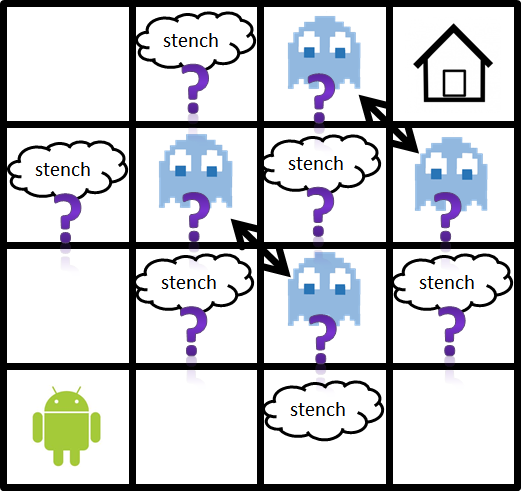
\includegraphics[scale=0.38]{Wumpus3.png}
\label{fig:wumpus}
}
\end{minipage}
\begin{minipage}{.6\textwidth}
\centering
\subfigure{
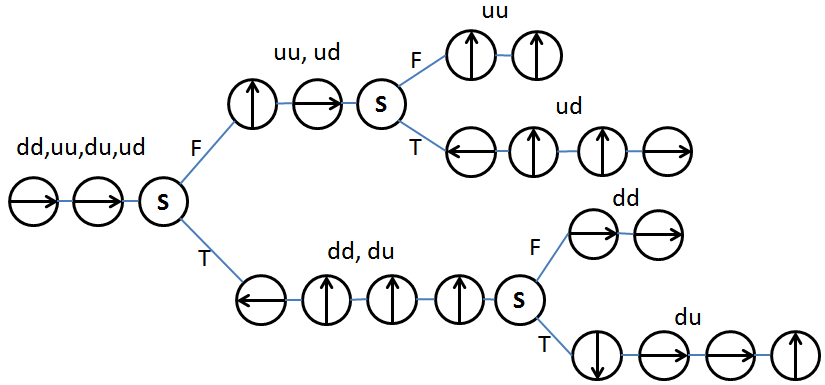
\includegraphics[scale=0.35]{PlanTree.png}
\label{fig:PlanTree}
}
\subfigure{
\centering
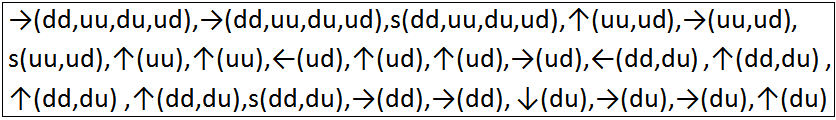
\includegraphics[scale=0.38]{LinearPlan.png}
\label{fig:LinearPlan}
}
\end{minipage}
\caption{The $4 \times 4$ Wumpus domain. A plan tree, with arrows denoting movement actions, {\em S} denoting sensing for stench, and outgoing edges marked by $T$ or $F$ (stench was observed or not). Branches are associated with the current possible belief state, i.e. set of possible states. A possible linearization of the plan tree. Actions are associated with the adequate belief state.}
\end{figure*}


\subsection{Knowledge and Its Evolution}
The belief state of the agent is what, in the traditional literature, is referred to as its set of possible worlds, or knowledge state~\citep{FHMV94}.
The knowledge of the agent corresponds to the facts that hold in all its possible worlds.
Essentially, this is the information it can deduce from its knowledge about the set of possible initial states of the world, the actions it  executed, and the observations it observed.

If some formula $\varphi$ is true in all states in the agent's current
belief state, we say that it knows $\varphi$, denoted $K\varphi$.
Initially, the agent's belief state, the set of currently possible states, is $b_I$. As it attains information, the size of this set decreases, because we can rule out initial
states that are inconsistent with its observations. Initial states that were ruled out due to inconsistency with some observation can never become ``possible'' again. If one maintains the initial belief state, and updates this representation each time a new observation is obtained \citep{SDR}, then the uncertainty over the initial belief and hence over the current belief state, i.e., the number of possible initial and current states given the observations, can only get reduced\footnote{This is true only for deterministic do. When actions have non-deterministic effects, the uncertainly may grow.}.

A major difficulty of contingent planning is that we cannot predict, at planning time, what will be observed following a sensing action. Thus, we cannot predict the agent's state of knowledge at run-time. At planning time, though, useful knowledge may be gained and leveraged.

First, if we know what actions were executed, we know whether the agent will know the value of certain facts.
Specifically, if the agent executes an action that observes the value of $p$, we know that, afterwards,  it will know the value of $p$, even though we do not know whether $p$ or $\neg p$ will be observed.
This knowledge can be represented by propositions of the form $KWp$ (\emph{know-whether} $p$).
\commentout{
Notice that if we know that the agent will
know the value of $p$ and we know that the value of $p$ is {\em true}, then we know that the agent will know "$p$  is true."
That is $KWp \wedge p \rightarrow Kp$.
}
Second, we can maintain specific information about the knowledge that the agent will
have following the execution of an action sequence, \emph{conditioned} on state $s$ being the true initial state.
If $s$ is the initial state, in a deterministic environment, we know what observations the agent will make,
and consequently, its state of information at run-time. In particular, given that $s$ is the true world state, we know which states
it will be able to distinguish from $s$ (because they would induce different observations), and which states it will not be able to distinguish from $s$ (because they would yield the same observations as $s$). Hence, we know the agent's future belief states, given that $s$ is the true initial state.

We assume here that for each pair of initial states $s_1,s_2$, either there exists some plan $\tau$ resulting in an observation $o$ that distinguishes between the states, or there exists some plan $\tau'$ that is applicable in both initial states and obtains the goal. Otherwise, no contingent plan solves the problem.


\section{The Multi-Path Translation}

We now suggest a method for translating contingent planning problems into classical planning problems whose
solution is (essentially) a contingent plan in linear form. There are two elements to this translation: a representation
of the knowledge state of the agent, and an enhanced actions set.

For representing knowledge we need 3 types of propositions: propositions that represent the current value of world features, conditioned upon an initial state, propositions that represent whether the agent currently knows the value of world features, given an initial state, and propositions that allow the reasoning about the belief state. For the latter, we maintain propositions that define whether two states $s$ and $s'$ are {\em distinguishable}, i.e., whether the agent has observed a proposition whose value is different in the two states.

We enhance the set of actions by adding, for each action $a$ and every possible belief state $b'$, an action
$a_{b'}$, that applies only if the current belief state is $b'$. The number of actions thus increases substantially, and we discuss practical solutions later.

Given the input problem $\pi=\langle P,A,\varphi_I,G\rangle$ and current belief state $b$ (at first, $b=b_I$), we generate a classical planning problem
$\pi_c = \langle P_c,A_c, I_c, G_c\rangle$ as follows:
\begin{description}
\item [Propositions] $P_c = \{p/s : p\in P , s\in b\}\cup \{KWp/s : p\in P , s\in b\}\cup\{KW\neg s/s' : s,s'\in b\}.$
\begin{enumerate}{\leftmargin=0em \itemindent=0em}
\item Propositions of the form $p/s$ capture the value at run time of $p$ when $s$ is the true initial state.
\item Propositions of the form $KWp/s$ capture the knowledge at run time regarding the value of $p$ when $s$ is
the true initial state. If $KWp/s$ holds, then the agent knows $p$'s value if $s$ is the true initial state (and
that value is the value of $p/s$).
\item When $\phi$ is a conjunction of literals, we write $\phi/s$ as a shorthand to $\bigwedge_{p \in \phi}p/s$, and we write $KW\phi/s$ as a shorthand to $\bigwedge_{p \in \phi}KWp/s$.
\item Propositions of the form $KW\neg s'/s$ denote that at run-time, if $s$ is the true
initial state, then the agent has gathered sufficient data to conclude that $s'$ cannot be the true initial state. These propositions allow us to define the belief state during execution. $KW\neg s'/s$ is reflective, i.e. $KW\neg s'/s$ iff $KW\neg s/s'$.
\end{enumerate}
\item [Actions] For every action $a\in A$, and every subset of $S'\subseteq b$, $A_c$ contains an action $a_{S'}$. This action
denotes the execution of $a$ when the agent's belief state is $S'$. $a_{S'}$ has no effect on states outside $S'$! It is defined as follows:
\item \emph{pre}($a_{S'}$) =  $\{KWp/s \wedge p/s : s \in S', p\in \mbox{\emph{pre}}(a)\} \cup\{KW\neg s'/s : s' \in S', s \in b\setminus S'\}$. That is, the agent must \emph{know} that the preconditions are true prior to applying the action in all states for which this action applies, {\em and} it must be able to distinguish between any state in $S'$ and every state {\em not} in $S'$. Thus, the agent can execute $a_{S'}$ only when it knows that the current belief state is $S'$, and all action preconditions are known to hold in $S'$.
\item For every $(c,e)\in $ \emph{effects}($a$), \emph{effects}($a_{S'}$) contains the following conditional effects:
\begin{enumerate}{\leftmargin=0em \itemindent=0em}
\item For each $s \in S'$, $(c/s,e/s)$ --- the effect applied to every state in $S'$.
\item $(\bigwedge_{s \in S'} KWc/s \wedge c/s, \bigwedge_{s \in S'} KWe/s)$ --- if we know that the condition $c$ holds prior to executing $a$ in all states for which the action applies, we know whether its effect holds following $a$.
\item $(\bigvee_{s \in S'} \neg KWc/s , \bigwedge_{s \in S'} \neg KWe/s)$ --- if we do not know whether the condition $c$ holds prior to executing $a$ in some of the states for which the action applies, we may not know whether its effect holds following $a$. This is a subtle point which we discuss later.
\item $\{KWp/s : p \in \emph{obs}(a), s \in S'\}$ --- for every observable $p$, we would know its value in all the states for which the action applies.
\item $\{(KWp/s \wedge KWp/s' \wedge p/s \wedge \neg p/s' , KW\neg s/s')\}$ --- for every observable $p \in obs(a)$, and every two states $s,s' \in S'$, if we know the value of $p$ in the two states, and both states disagree on $p$, then we can distinguish between the states at runtime.
\end{enumerate}

\item In addition, for each literal $l$ (w.r.t.~$P$) and each subset of states $S' \subseteq b$ we have a merge action that allows us to gain knowledge:
\begin{list}{$\bullet$}{\leftmargin=0em \itemindent=0em}
\item \emph{pre}(merge($l,S'$)) = \\$\{\bigwedge_{s \in S'}l/s\} \wedge \{\bigwedge_{s' \in S', s \in b\setminus S'} KW\neg s/s'\}$ --- the merge can be used when all states in $S'$ agree on the value of $l$, and we can distinguish at run time between the states in $S'$ and the rest of the states.
\item \emph{effects}(merge($l,S'$)) = \{$KWl/s : s \in S'$\} --- the effect is that we now know whether $l$ holds in all these states.
\end{list}

\item [Initial State] $I_c = \bigwedge_{s\in b,s\models l} $ $l/s$ --- for every literal we specify its value in all states.
\item [Goal] $G_c = \{\bigwedge_{s \in b} G/s \}$ --- we require that the goal will be achieved in all states.
\end{description}

The reader may have observed that the merge actions are powerful. If we correctly keep track
of the value of every proposition given every possible initial state, and the value of propositions of the form
$KW\neg s'/s$, we can infer any propositions of the form $KWp/s$ that is currently true.
Keeping track of basic ($p/s$) propositions is easy, and keeping track of $KW\neg s'/s$ propositions is also easy:
they never become false --- new observations can only cause us to distinguish between more states.
This implies that, in principle, we can offer an even simpler, sound and complete translation, in which none of the
non-merge actions adds knowledge about the value of the propositions (i.e., propositions of the form $KWp/s$), and all such knowledge is removed after every action.
However, this would require much longer plans that contain many merge actions, in order to recover the lost knowledge.
Instead, we conservatively update the agent's knowledge via regular actions. Any missing information, can be
deduced with the merges. These observations underlie the soundness and completeness result below.

It is always beneficial to apply merge actions when possible, because merge actions are internal actions which can be considered to be costless for the agent. Thus, it is better to acquire information through merge actions rather than through sensing actions. In fact, many planners support axioms, which are automatically executed whenever possible, which is suitable for the merge actions.

\begin{theorem}
$\pi$ has a contingent plan IFF $\pi_c$ has a plan.
\end{theorem}
\proof (outline) Having established the relation between plan trees and their linearizations,
the main observations upon which this result builds are (1) The classical plan correctly maintains the actual state of the world
for every possible initial state (using the propositions $p/s$). (2) The classical plan correctly and completely tracks the set of
distinguishable state (i.e., propositions of the form $KW\neg s'/s$).
(3) One can use the merge actions to deduce any valid proposition of the form $KWp/s$.
(4) All conclusions of the form $KWp/s$ added by a non-merge action are sound.
\qed

  \begin{algorithm}[h!]
\scriptsize
    \caption{MPSR}
    \label{planner}
\begin{algorithmic} %[n] = every n'th line is numbered
      \REQUIRE Contingent Planning Problem: $\pi= \langle P,A,\varphi_I,G \rangle$, Integer: \emph{size}
      \STATE $b :=  $initial belief state
      \STATE \emph{changed} :=\emph{ false}
      \WHILE {$G$ is not known at the current belief state}
        	\STATE Sample a  set of states $S'_I$ consistent with $b$ s.t. $|S'_I|\leq$\emph{size}
	\STATE $\rho$ := (linear) solution to $\langle P,A,S'_I,G\rangle$ using the multi-path translation.
	\IF {$\rho$ is empty}
	\RETURN failure
	\ENDIF
	\WHILE {$ \rho\neq\emptyset$ and \emph{not} \emph{changed} and \emph{pre}(first($\rho$)) is known at the current belief state}
		\STATE $a :=  $first($\rho$)
		\STATE execute $a$, observe $o$
	       	\STATE $b_{new} :=  \{ a(s) : s\in b\ and\ s\models o\}$
		\STATE \emph{changed} := $[b \neq b_{new}]$
		\STATE Remove $a$ from $\rho$
	\ENDWHILE
    	\ENDWHILE
    \end{algorithmic}
  \end{algorithm}

\subsubsection{Translations Linear in $|b|$}

The above translation adds a number of actions exponential in the number of initial states, and potentially, doubly exponential
in the number of propositions. However, there exists an alternative translation that, like previous complete translations
for conformant planning, is linear in the number of initial states, and hence only worst-case exponential in the number of propositions.
We define one action $a_s$ for each original action $a$ and possible initial state $s$. This action $a_s$ applies $a$ to all
states that are currently indistinguishable from state $s'$, where $s'$ is the state obtained by applying the current plan prefix to initial state $s$.
This translation exploits the fact that the number of possible belief states after each plan prefix is at most $|b_I|$.
Yet, although this translation introduces a linear number of new actions, these actions require many conditional effects.
Such actions are challenging for current classical planners. Thus, given the fact that after sampling (Section~\ref{scn:Sampling}) we consider only a
small number of initial states, we use the former translation, which is more effective in practice.

\section{The Multi-Path Planning Algorithm}

The multi-path translation allows us, in principle, to solve any contingent planning problem with a classical planner.
However, this approach is impractical for two reasons. First, complete plans (trees) are very large. Generating
them offline is, thus, difficult, and recent work has moved towards online planning, in which the planner generates
a single execution sequence. Second, our translation is linear in the number of possible initial states, and hence exponential in the number of propositions --- due to the
need to maintain propositions for each possible world state.
One can slightly improve the situation by using tags, denoting sets of states, rather than actual states, as
introduced by~\citet{PalaciosG09}, but even with tags the size of the translation can be unmanageable~\citep{SDR}. Instead, we take a sampling and replanning approach in the spirit of the SDR planner~\citep{SDR}.

\subsection{Replanning with MPSR}

MPSR (for multi-path, sampling, replanner)
is an online contingent planner that uses a replanning approach.
MPSR maintains the agent's current belief state using the lazy method introduced in SDR. At each
iteration MPSR generates a multi-path translation using only a small subset of $b_I$ --- typically of size no greater than 4.
The resulting plan is typically not a solution plan because some possible initial states were ignored.
However, it is much more informed than plans generated using single-execution path methods, such as SDR.
MPSR executes the plan until either a new observation is made, which alters the belief state, or the next
action is not safe to execute because its preconditions do not hold in one of the possible states. Then, it replans again.
The high level scheme of MPSR  is described in Algorithm~\ref{planner}.
\emph{size} controls the size of the set of world states $S'_I$.


For belief maintenance and update we use the lazy regression technique suggested by \citet{SDR}, where only the initial belief state is maintained, and queries concerning possible current states are resolved by regressing the query through the action-observation history.

\subsection{Sampling and Resampling}
\label{scn:Sampling}

\begin{algorithm}[ht]
    \caption{Diverse-Sampling}
    \label{alg:sampling}
\scriptsize
  \begin{algorithmic}
      \REQUIRE $\varphi$ --- the constraints over the belief state, $size$
      \STATE $P \leftarrow$ all unknown predicates in $\varphi$
      \STATE $S \leftarrow \emptyset$, $P' \leftarrow P$, $\varphi' \leftarrow \varphi$, $s \leftarrow \emptyset$
      \WHILE{$P' \neq \emptyset$}
      \STATE Choose $p \in P', l \in \{p, \neg p\}$ uniformly
    \STATE Propagate $l$ through $\varphi'$
     \STATE \textbf{if} $\varphi'$ is solvable \textbf{then} add $l$ to $s$ \textbf{else} backtrack
        \STATE $P' \leftarrow$ all unknown predicates in $\varphi'$
      \ENDWHILE
      \STATE Add $s$ to $S$, $s \leftarrow \emptyset$
      \WHILE{$|S|<size$}
       \STATE $P' \leftarrow P$, $\varphi' \leftarrow \varphi$
      \WHILE{$P' \neq \Phi$}
      \STATE Choose $p \in P', l \in \{p, \neg p\}$ s.t. $l$ does not appear in $S$. If no such $l$ exists, pick $p,l$ uniformly.
    \STATE Propagate $l$ through $\varphi'$
     \STATE \textbf{if} $\varphi'$ is solvable \textbf{then} add $l$ to $s$ \textbf{else} backtrack
      \STATE $P' \leftarrow$ all unknown predicates in $\varphi'$
      \ENDWHILE
      \STATE Add $s$ to $S$
      \ENDWHILE
      \RETURN $S$
    \end{algorithmic}
   \end{algorithm}

To improve the value of the plan generated by multi-path translation, we would like to sample a diverse set of states.
There are different ways to define diversity in this context. Our sampling algorithm (Algorithm~\ref{alg:sampling})
seeks to find a set $S$ of possible initial states of predefined size, such that the number of propositions $p$
that attain different values on state in $S$ is maximized (i.e., there exists states $s',s''\in S$ such that $s'\models p$ and $s''\models\neg p$).

We use the following technique to obtain a diverse sample (Algorithm~\ref{alg:sampling}):
We  sample an unknown proposition, assign it a value, and propagate this assignment through the belief state constraints, setting the values of other dependent propositions. We continue to sample  this way
until all propositions have been assigned. For the rest of the states, whenever we need to pick a proposition to assign,
we seek a proposition that was assigned uniformly in all samples, so far.
We assign it the complementary value, propagate its value, and continue. If all
remaining literals have diverse values in the states assigned so far, we continue sampling arbitrary unassigned propositions,
as before.
Diverse sampling is an important component of MPSR, but given the small sample size that we use, we may not be able to cover all aspects of
the initial state. To get a more informed plan, we use resampling.
That is, we generate $m$ initial state sets $S_1,S_2,...,S_m$, all of which contain only a small number of states. We then plan for each $S_i$ independently, resulting in a plan $\pi_i$. As computing $m$ plans with a sample size $n$ is (much) faster than solving a single plan with sample size $n+1$, this approach scales better than increasing the sample size.
Then, we select the plan that applies a sensing action the earliest. This usually indicates an awareness to conflicting needs that can be resolved by sensing.
\section{Empirical Evaluation}
We now compare MPSR to CLG~\citep{AlborePG09} and SDR* --- the best variation of SDR~\citep{SDR}, on benchmarks from the SDR paper. These are currently the best contingent planners. We evaluate MPSR using a single sample, denoted MPSR, and MPSR using resampling with $5$ samples, denote MPSR $\times 5$. MPSR  always uses two sampled states. The experiments were conducted on a Windows Server 2008 machine with 24 2.66GHz cores (although each experiment uses only a single core) and 32GB of RAM. The underlying planner is FF ~\citep{hoffmann:nebel:jair-01}.

\begin{table*}[htb]
\centering
\caption{
\footnotesize
Comparing MPSR to CLG (execution mode) and SDR* --- the best SDR variation in each domain. For do with conditional actions (\emph{localize}) CLG execution cannot be simulated. We denote {\em TF} when the CLG translation failed, {\em CSU} when CLG  cannot run a simulation with a uniform distribution, and {\em PF} where the CLG planner failed, either due to too many predicates or due to timeout. Do were FF was unable to solve the translation are denoted by {\em FFF}. Values in parentheses denote standard error. Maximum time allowed was 30 minutes. Best time and plan length for each domain are bolded.
}
\scriptsize
\begin{tabular}{|l||l|l||l|l||l|l||l|l|}
\hline
	&\multicolumn{2}{c||}{MPSR}&\multicolumn{2}{c||}{MPSR $\times$ 5}&\multicolumn{2}{c|}{SDR*}&\multicolumn{2}{c|}{CLG}\\\hline
Name	&	\#Actions			&	Time(secs)			&	\#Actions			&	Time(secs)			&	\#Actions			&	Time(secs)			 &	\#Actions		 &		Time(secs)		\\ \hline
cloghuge	&		FFF&		&		FFF		&		&		61.17	(	0.44	)&	117.13	(	4.19	)&		\textbf{51.76}	(	0.33	)&	\textbf{8.25}	(	 0.08	 )\\
ebtcs-70	&	44.5	(	0.7	)&	22.4	(	0.3	)&			\textbf{37.2}	(	0.8	)&	12.8	(	0.3	)&		\textbf{35.52}	(	0.75	)&	\textbf{3.18}	(	 0.07	)&		\textbf{36.52}	 (	0.86	)&	73.96	(	0.14	 )\\
elog7	&	23.5	(	0.1	)&	1.4	(	0.1	)&			22.4	(	0.1	)&	3.8	(	0.1	)&		21.76	(	0.07	)&	\textbf{0.85}	(	0.01	)&		\textbf{20.12}	 (	0.05	)&	1.4	(	0.08	 )\\
\hline

CB-9-1	&	359.1	(	3.9	)&	\textbf{61.1}	(	1.3	)&			188.9	(	3.9	)&	\textbf{61.1}	(	1.3	)&		124.56	(	2.49	)&	71.02	(	1.57	)&		 \textbf{94.36}	(	1.83	 )&	129.3	(	0.26	 )\\
CB-9-3	&		FFF&		&				FFF&		&		\textbf{247.28}	(	2.91	)&	\textbf{245.87}	(	4.03	)&		\textbf{252.76}	(	2.66	)&	819.52	 (	0.47	)\\
CB-9-5	&		FFF&		&				FFF&		&		\textbf{392.16}	(	2.81	)&	\textbf{505.48}	(	8.82	)&		PF			&				\\
CB-9-7	&		FFF&		&				FFF&		&		\textbf{487.04}	(	2.95	)&	\textbf{833.52}	(	15.82	)&		PF			&				\\
\hline

doors5	&	17.24	(	0.2	)&	\textbf{2}	(	0.1	)&			\textbf{15.8}	(	0.2	)&	5.8	(	0.1	)&		18.04	(	0.18	)&	\textbf{2.14}	(	0.03	)&		 16.44	(	0.18	)&	2.4	 (	0.1	)\\
doors7	&	40	(	0.4	)&	\textbf{6.5}	(	0.1	)&			34.2	(	0.3	)&	16.4	(	0.2	)&		35.36	(	0.41	)&	9.29	(	0.1	)&		\textbf{30.4}	 (	0.24	)&	20.44	(	 0.02	)\\
doors9	&	67.12	(	0.7	)&	\textbf{17.8}	(	0.2	)&			53.92	(	0.5	)&	42.7	(	0.4	)&		51.84	(	0.55	)&	28	(	0.31	)&		 \textbf{50.48}	(	0.5	)&	38.52	(	 0.06	)\\
doors11	&	117.8	(	1	)&	\textbf{48.8}	(	1.4	)&			75.68	(	0.6	)&	99.2	(	0.8	)&		88.04	(	0.91	)&	79.75	(	1.04	)&		 \textbf{71.68}	(	0.79	)&	 126.59	(	0.1	)\\
doors13	&	197.92	(	1.2	)&	\textbf{105.5}	(	2.1	)&			140.12	(	1	)&	249.1	(	3.2	)&		120.8	(	0.93	)&	158.54	(	2.01	)&		 \textbf{105.48}	(	0.89	)&	 330.73	(	0.21	 )\\
doors15	&	262.2	(	1.9	)&	\textbf{190}	(	3.3	)&			167.8	(	1.6	)&	418.5	(	6.1	)&		\textbf{143.24}	(	1.36	)&	268.16	(	3.78	)&		 PF			&				 \\
doors17	&	368.25	(	3.4	)&	\textbf{335.3}	(	5.3	)&			221.4	(	2.2	)&	686.6	(	11.4	)&		\textbf{188}	(	1.64	)&	416.88	(	6.16	)&		 PF			&				 \\
\hline

localize3	&	8.1	(	0.1	)&	\textbf{1.2}	(	0.1	)&			\textbf{7.2}	(	0.1	)&	2.1	(	0	)&		8	(	0.12	)&	1.77	(	0.03	)&		CSU&	 \\
localize5	&	16	(	0.3	)&	\textbf{1.5}	(	0.1	)&			15.5	(	0.3	)&	4.1	(	0.1	)&		\textbf{14.56}	(	0.24	)&	7.12	(	0.1	)&		CSU&	 \\
localize9	&	30.7	(	0.4	)&	\textbf{11.1}	(	0.2	)&			33.1	(	0.5	)&	25.6	(	0.5	)&		\textbf{28.52}	(	0.42	)&	72.69	(	1.43	)&		 CSU&	\\
localize11	&	38.5	(	0.6	)&	\textbf{31.1}	(	1.4	)&			39.9	(	0.6	)&	71.3	(	1.4	)&		\textbf{34.67}	(	0.61	)&	155.6	(	3.87	)&		 PF			&	\\
localize13	&	42.4	(	0.8	)&	\textbf{73.4}	(	1.9	)&			47.2	(	0.8	)&	185.4	(	5	)&		\textbf{37.52}	(	0.62	)&	396.76	(	10.72	)&		 PF			&		\\
localize15	&	45	(	0.9	)&	\textbf{130.6}	(	4.1	)&			59.8	(	1.1	)&	384.9	(	8	)&		\textbf{40.08}	(	0.61	)&	667.22	(	19.7	)&		 PF			&				 \\
localize17	&	59.8	(	0.9	)&	\textbf{230.4}	(	7.7	)&			71.8	(	1.1	)&	687.4	(	15.3	)&		\textbf{45.00}	(	0.86	)&	928.56	(	33.2	 )&		PF			&				 \\
\hline

unix1	&	\textbf{9.8}	(	0.2	)&	0.6	(	0.1	)&			10.8	(	0.1	)&	0.9	(	0	)&		12.2	(	0.16	)&	0.48	(	0.01	)&		11.68	(	 0.23	)&	\textbf{0.35}	(	 0.01 )	\\
unix2	&	30.6	(	0.6	)&	\textbf{1.9}	(	0.1	)&			24.9	(	0.4	)&	3.9	(	0.1	)&		26.44	(	0.72	)&	1.41	(	0.03	)&		 \textbf{19.88}	(	0.47	)&	2.69	 (	0.01	)\\
unix3	&	69.7	(	1.7	)&	\textbf{5.2}	(	0.1	)&			\textbf{51.7}	(	1.1	)&	13	(	0.2	)&		56.32	(	1.72	)&	\textbf{5.47}	(	0.18	)&		 \textbf{51.32}	(	0.97	 )&	18.56	(	0.05	)\\
unix4	&	158.6	(	4.3	)&	\textbf{30.4}	(	1.1	)&			138.1	(	3.6	)&	61.8	(	1.2	)&		151.72	(	4.12	)&	35.22	(	0.94	)&		 \textbf{90.8}	(	2.12	)&	 189.41	(	0.6	)\\
\hline

Wumpus05	&	\textbf{23.4}	(	0.2	)&	4.5	(	0	)&			\textbf{23.0}	(	0.2	)&	7.1	(	0.1	)&		34.72	(	0.3	)&	6.51	(	0.07	)&		24.12	 (	0.1	)&	\textbf{2.38}	 (	0.09	)\\
Wumpus10	&	47.2	(	1	)&	\textbf{12.4}	(	0.2	)&			44.2	(	0.4	)&	23.1	(	0.2	)&		70.64	(	1.13	)&	65.89	(	1.13	)&		 \textbf{40.44}	(	0.18	)&	 36.29	(	0.04	 )\\
Wumpus15	&	\textbf{65}	(	1.6	)&	\textbf{126.6}	(	3.1	)&			\textbf{67.2}	(	0.8	)&	262.7	(	5	)&		120.14	(	2.4	)&	324.32	(	7.14	)&		 101.12	(	0.67	)&	 330.54	(	0.25	 )\\
Wumpus20	&	\textbf{71.6}	(	1.2	)&	\textbf{261.1}	(	7	)&			79.9	(	0.9	)&	773.6	(	7.9	)&		173.21	(	3.4	)&	773.01	(	20.78	)&		 155.32	(	0.95	)&	1432	 (	0.47	 )\\
\hline
\end{tabular}
\label{tbl:Results}
\end{table*}

Table~\ref{tbl:Results} shows that MPSR is typically faster than all other planners. When resampling is used,  planning time increases, but plan quality (number of actions) typically improves. In \emph{localize}, MPSR does not offer better plan quality than SDR because in this domain the best behavior is to guess a possible state and plan for it. In \emph{colorballs} (CB) and the larger logistics domain (\emph{cloghuge}), the underlying FF planner failed to solve the translated do, possibly because the resulting plan trees are huge. In Wumpus, MPSR generates much better plans, much faster than either SDR or CLG.


To demonstrate where MPSR overcomes the disadvantages of SDR, we experiment on a Wumpus variation with deadends.
Wumpus requires a smart exploration and sensing policy, and is thus one of the more challenging benchmarks. Originally, the agent requires a cell to be ``safe'' before entering it. We removed this precondition, and changed the move action so that the agent is dead if it enters a cell containing a wumpus or a pit, creating deadends. As expected SDR and all its variations fail utterly. CLG, however, solves these do without failing. MPSR can rapidly solve this domain with good quality plans. MPSR uses 3 initial states, that given our diverse sampling technique, cover all possible safe configurations. We note that this is a fairly simple type of deadend, that is easily detected and handled. In general, MPSR sampling technique can still be trapped by more sophisticated deadends.


\begin{table}[htb]
\centering
\caption{
\small
Wumpus do with deadends. TF denotes that the CLG translation did not complete in 30 minutes.}
\scriptsize
\begin{tabular}{|l||l|l||l|l|}
\hline
	&  \multicolumn{2}{c||}{MPSR} &	\multicolumn{2}{c|}{CLG}	\\ \hline
Name & Time (secs) & \#Actions&  Time (secs) & \#Actions \\
\hline
Wumpus 4 & 1.3 (0.01)& 17.5 (0.1) & 0.17 (0.001) & 17.7 (0.04) \\
Wumpus 8 & 16.9 (1.5)& 27.5 (1.1) & 2.8 (0.01) & 40.5 (0.31) \\
Wumpus 16 &93.5 (4.5) &38.3 (1.2) &  182.5 (1.73) & 119.7 (0.91) \\
Wumpus 20 &216.8 (6.7) &48.28 (1.2) & TF & \\
Wumpus 24 &285.5 (5.5) &71.5 (0.7) &  TF &  \\
\hline
\end{tabular}
\label{tbl:Deadends}
\end{table}




\section{}

We introduced a new translation scheme from contingent planning into classical planning. The method is sound and complete, but comes at substantial cost --- the resulting plans can be very large. This cost can be controlled by selective sampling of the initial states combined with replanning, as we did here, or by using the multi-path translation as a method for generating informed heuristic estimates. Our empirical evaluation shows that MPSR is typically faster than SDR and CLG,
although its plans are longer, but that on the  

ministic effects. The multi-path formulation is partly motivated by the difficulty of current methods to deal with non-deterministic effects. This difficulty has two -  (when possible) in later stages when effects are not as  help. The second difficulty is technical. All translation       ~\citet{PalaciosG09}, which is well suited  a  

     


%---------------------------
%   acknowledgement
%---------------------------
\noindent {\bf Acknowledgement:} Ronen Brafman is partially supter   
%----------------------
%   bibliography
%----------------------

\small
\bibliographystyle{aaai}   %Declare which Bibliography style (file) to use
\clearpage
\bibliography{all}   %The .bib file to use, no need to include the file extension



\end{document}



